\section{Overview}
We explain the operation of a two-party state channel and then extend the functionality to multiple parties. A data structure that models the cash distribution after each hand is introduced. Lastly, a leave protocol is described that protects participants from accepting uncovered bets. 


\subsection{State Channels}
State channels are a way to think about blockchain interactions which could occur on-chain, but instead get conducted of the chain, without  increasing the risk of any participant. The most well known example of this strategy is the idea of payment channels in Bitcoin, which allow for instant fee-less payments to be sent directly between two parties \cite{coleman15}. 

The life-cycle of a state channel can be broken down into steps as depicted in figure \ref{pc_settle}:

\begin{figure}[!ht]
\centering
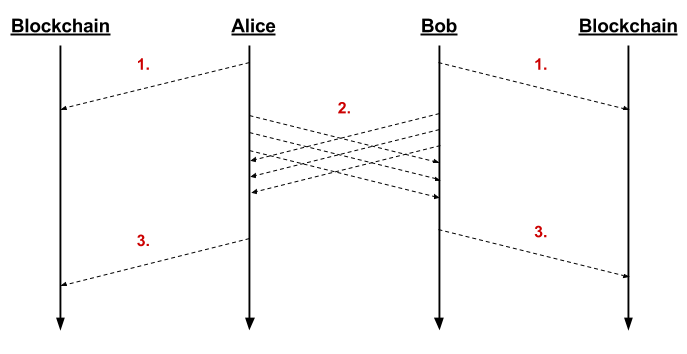
\includegraphics[width=3.0in]{images/settle.png}
\caption{A state channel settled in agreement.}
\label{pc_settle}
\end{figure}

\begin{enumerate}
\item Alice and Bob lock up some tokens or a state description they control.
\item They can internally do transactions by signing receipts about new commitments and exchanging them. The receipts have to carry strictly increasing sequence numbers and signatures.
\item Alice and Bob can release the bonded tokens by mutually agreeing (signing) on a resolution.
\end{enumerate}

Obviously, there is a possibility that Alice and Bob will not agree in all situations. In figure \ref{pc_dispute} the dispute case is depicted:

\begin{figure}[!ht]
\centering
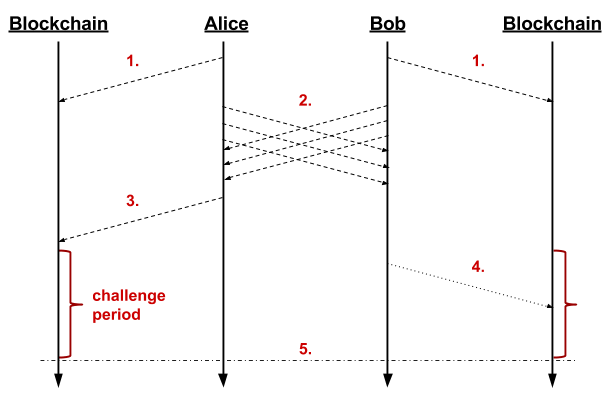
\includegraphics[width=3.0in]{images/dispute.png}
\caption{A state channel settled after dispute.}
\label{pc_dispute}
\end{figure}

\begin{enumerate}
\item Alice and Bob lock up some tokens or a state description they control.
\item They can internally do transactions by signing receipts about new commitments and exchanging them. The receipts have to carry signatures and strictly increasing sequence numbers.
\item If Alice or Bob stop cooperating, the latest receipt can always be written on the blockchain. This will trigger a challenge period.
\item During this period a newer receipt (higher nonce) can be submitted.
\item After the challenge period expires, the bonded tokens are released to Alice and Bob by the ratio of the highest receipt.
\end{enumerate}

In effect, a state channel buffers the operations that would otherwise be written to the blockchain. This decouples the application using a state channel from the liveliness constraints of the blockchain without relaxing the security assumptions.

\subsection{Multi-party State Channels}

An interaction of multiple participants could be modeled as a set of bilateral state channels from each player to each player. Yet, as the distribution of cash is not known beforehand, each channel would need to be funded with the full amount, resulting in a requirement of security deposits of O(n\^2) tokens.

To be able to operate the channel with multiple parties and O(n) size of deposits, we define a commitment data structure as shown in figure \ref{mpc_round}. 

\begin{figure}[!ht]
\centering
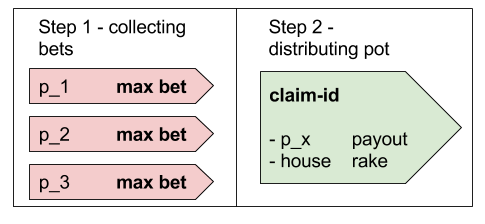
\includegraphics[width=2.5in]{images/bet.png}
\caption{Commitments and distribution}
\label{mpc_round}
\end{figure}

Commitments by participants carry a value, but do not have a specific recipient. Each higher value commitment by a participant replaces a lower one. When results of secure computation become available an oracle evaluates the data and issue a corresponding distribution receipt, reassigning the values from the participants' commitments to the winner(s) deducted from the MPC.

Multiple rounds of commitments and distributions (hands played) can happen among the participants of the multi-party state channel. Figure \ref{mpc_settle} depicts that, as long as all parties agree on a final settlement, the protocol is similar to the two-party channel:

\begin{figure}[!ht]
\centering
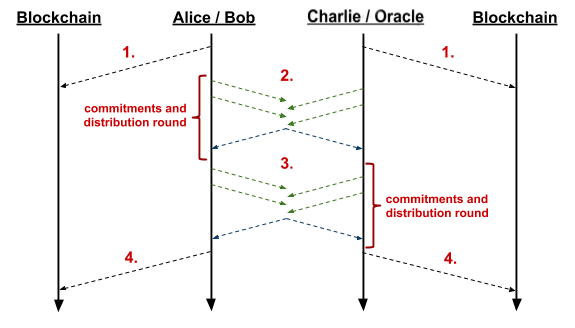
\includegraphics[width=3.0in]{images/multiSettle.png}
\caption{A multi-party state channel settled in agreement.}
\label{mpc_settle}
\end{figure}

\begin{enumerate}
\item Alice, Bob and Charlie lock up some tokens under their control.
\item They can internally do transactions by signing receipts about new commitments and exchanging them. The receipts have to carry signatures, an Id for the hand and increasing values.
\item They can have multiple rounds of commitment and distribution with a strictly increasing identifier.
\item Alice, Bob and Charlie mutually agree on a resolution. They sign the resolution after each validating the sum of all value transferred. The smart contract evaluates the resolution and releases the bonded tokens.
\end{enumerate}

In a dispute case when no resolutions can be found, parties can start submitting receipts of commitments and distributions. Naturally, participants are incentivised to collect receipts in those rounds where they have a share in the distribution to submit them in the dispute case.

In the dispute period commitment receipts with higher values can overwrite those with lower value and distribution receipts with higher claimId overwrite those with lower one.

After the challenge period expires, all receipts are simply summed up on the chain and the bonded tokens are released according to the resulting balances.

\subsection{P2P book keeping}

A participant can sign a commitment of any size, participants have to check by looking at deposit and summing up all previous commitments and distributions to see if commitment doesn't exceed deposit.

\subsection{Asynchronous participation}

Rotation into a state channel requires no special protocol, once the deposit is placed, the participant can be interacted with.

Rotation of of a channel has the potential risk that a remaining party could be handed uncovered commitments by the leaving party after it has withdrawn its deposit already. To guard against this situation, we extend the on-chain state with the variables:

lastHandNetted: describes the id of the last hand at which the channel has been netted. this is also the hand at which the balance of the participant is valid.

exitHand: each participant maintains this flag, which is initialized with 0 and stays unchanged until the participant signals to leave. At that point the participant requests a leave receipt from the oracle, which identifies the latest hand id in the channel. This receipt is submited to the chain and sets the exit Hand of the participant.

lastHandNettingRequest: this is either lastHandNetted or a higher id, if the channel is in dispute.

Once the exitHand flag of a leaving participant is set on chain, other participants can clearly judge to accept or reject receipts based on their hand id. When, either through agreement, or dispute, lastHandNetted is increased to equal or beyond a participants exitHand id, the participant is payed out and removed from the channel. 
